\chapter{Network Layer\label{chap:networklayer}}
Die Aufgabe des Networklayers ist es Nachrichten durch das Netz zu Routen. Ausserdem ist der Networklayer dazu zuständig Positionsinformationen des Fahrzeuges an seine Umgebung zu senden. Dieser Vorgang wird als beaconing bezeichnet. Dabei werden periodisch kleine Pakete an die Umgebung versendet. Diese Daten werden von jedem Fahrzeug in zwei Tabellen verwaltet. Eine dieser beiden Tabellen wird als neighbors table bezeichnet und enthält alle Informationen über die aktuellen Nachbarn. Die andere Tabelle heisst location table und verwaltet die Daten über Fahrzeuge die bekannt sind. Die Tabellen müssen andauernd aktualisiert werden was durch das beaconing erreicht wird.

\section{Congestion Control\label{sec:congestioncontrol}}
\todo{Hier nochmal nachhacken ob es tatsächlich keine lösung gibt}
Noch ungeklärt sind die Transport- und Überlastungskontrolle. Offen sind Fragen bzgl. fehlerfreiem Transport (single protocol/multiple protocols), Prioritäten von Datenpacketen, Datenaggregation und Payloadgröße. Ausfallsicherheit (connection-free/conncetion-less), Forwarding (end-to-end Prinzip), Transportarten (unicast/broadcast), Fairness, Komplexität, Multiplexing sowie Verzögerungen und Ortsgültigkeit sind auch zu klären.Es bleibt abzuwarten, wie mit den Problemen umgegangen wird. Auf Grund der vielen Anforderungen muss höchste Sorgfalt in die Entwicklung gelegt werden. Eine Herausforderung ist z.B. die Frage der Ortsgültigkeit. Unter Ortsgültigkeit ist zu verstehen, wie lange eine Nachricht in einer bestimmten Region bei der sich schnell ändernden Netzwerktopologie gültig bleibt, oder als veraltet verworfen wird.

\section{Geo Routing\label{sec:georouting}}
\subsection{Allgemein}
Da sich die Fahrzeuge andauernd mit hoher Geschwindigkeit bewegen und sich dadurch die Topologie des Netzes ständig ändert (Ad Hoc-Eigenschaft), muss definiert werden wie die einzelnen \acro{its} miteinander Kommunizieren können. Dazu wird das GeoNetwork spezifiziert. Um ein Fahrzeug bzw einen \acrol{GAR} anzusprechen, muss jeder \acrol{GAR} über eine GeoNetworking Adresse verfügen über die dieser erreicht werden kann. 

\subsection{\acrol{GNW} Adresse}
Die \acrol{GNW} Adresse besteht aus acht Bytes die verschiedene Informationen repräsentieren. Die ersten zwei Bytes werden zeigen ob die Adresse manuell oder Automatisch konfiguriert wurde, um was es sich für ein Fahrzeug handelt und ITS-S Country Code. Die restlichen sechs Bytes sind die eigentliche Adresse.
\todo{das versteh ich noch nicht ganz ipv6 hat doch 128bit?}
In order to allow for the resolution of a GeoUnicast destination GN_ADDR from an IPv6 destination address using virtual interfaces of type Ethernet V2.0/IEEE 802.3 LAN [i.12], the GeoNetworking address space shall remain 48-bit wide (size of the MID field in the GeoNetworking address). In particular, as described in ETSI EN 302 636-6-1 [6], table 1, note 1, the GN6ASL resolves an MID from a unicast destination IPv6 address and passes it to GeoNetworking via the service primitive GN-DATA.request (clause I.2). Then, the GeoNetworking protocol is responsible for deriving a full GN_ADDR from the MID. This full GN_ADDR shall be derived from a LocTE (if it exists) or by executing the Location Service with Request GN_ADDR field containing only the MID part and the other bits set to 0.
To be compliant with the IPv6 over GeoNetworking architecture, the GeoNetworking address space shall remain 48-bit wide (size of the MID field in the GeoNetworking address) in order to provide a virtual interface of Ethernet type to IPv6 layer and to perform the forwarding via GeoNetworking in a transparent way (see ETSI EN 302 636-6-1 [6]).
If the address is updated for privacy reasons, i.e. by assignment of an alias identity, only the last field of the address shall be updated and derived from the alias identity (pseudonym, see ETSI TS 102 731 [i.3]).
\subsubsection{Konfiguration der Adressen}
\todo{siehe etsi Kapitel 9.2.1 duplicate address detection ist auch interessant}
\subsection{Beaconing und Location Service}
\todo{siehe etsi kapitel 9.2.3/4}

\subsection{location- und neighbors table}
\todo{etsi 7.1 da steht was da alles drin ist}


\subsection{Geo Unicast}
Um einen einzelnen Knoten zu Adressieren wird der Geo Unicast spezifiziert. Die Autos die zwischen Sender und der Empfangseinheit liegen dienen als Zwischenstationen. Über den Geo Unicast werden Nachrichten entweder über einen Hop an das Ziel gesendet oder über Zwischenstationen mit mehreren Hops. Die Nachricht kann bei den Zwischenstationen verändert werden. Das heisst zwei oder mehr Nachrichten werden zu einer zusammengefasst bevor sie weitergesendet werden. Dieser Vorgang ist auch umgekehrt durchführbar, sodass eine Nachricht aufgeteilt werden kann. Der Inhalt der Nachricht kann ebenfalls verändert oder Informationen hinzugefügt werden. 

\begin{figure}
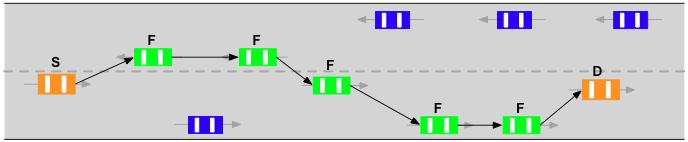
\includegraphics[width=0.99\textwidth]{content/images/03_networklayer/GeoUnicast.jpg}
\caption{Geo Unicast \cite{etsi102636-1}}
\label{fig:geounicast}
\end{figure}

\subsection{Topologically-scoped broadcast}
Der Topologically-scoped broadcast sendet einen Nachricht mit einem bestimmten Hop Count an alle um den Knoten erreichbaren Einheiten. Diese Nachricht wird dann von den Knoten empfangen, bei denen der Hop Count endet.

\begin{figure}
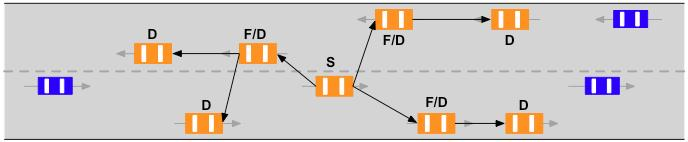
\includegraphics[width=0.99\textwidth]{content/images/03_networklayer/TSC.jpg}
\caption{Topologically-scoped broadcast mit Hop Count 2 \cite{etsi102636-1}}
\label{fig:tsc}
\end{figure}


\subsection{Geographically-scoped broadcast}
Über den Geographically-scoped broadcast ist es einem Knoten möglich, um sich herum oder in einer bestimmten Entfernung zu sich selbst eine definierte Region zu erreichen. 

\begin{figure}
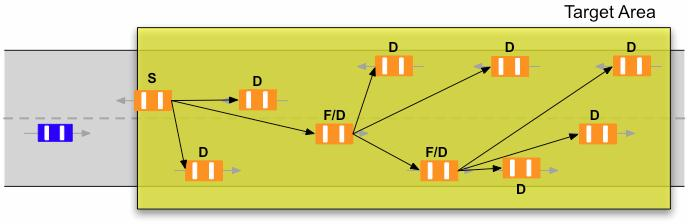
\includegraphics[width=0.99\textwidth]{content/images/03_networklayer/GSB.jpg}
\caption{geographically-scoped broadcast \cite{etsi102636-1}}
\label{fig:gsb}
\end{figure}
